\chapter{Installation on Unix platform}\label{sec:InstallUnix}

\paragraph{}The FA$\mu$ST project is based on \textbf{C++ library} available for Linux, MAC OS X and Windows platforms. The proposed toolbox provides a Matlab wrapper. \textbf{CMake} has been chosen to build the FA$\mu$ST project because it is an open-source, cross-platform family of tools designed to build, test and package software. This chapter presents the steps to install the FA$\mu$ST tools on Unix platform (both Linux and Mac OS). 

\paragraph{}Firstly, please ensure that the \textbf{prerequisites components} listed in Section \ref{sec:RequiredTools} are installed. Secondly, refer to section 
\ref{sec:UnixBuildDownload} to download FA$\mu$ST package and setting your terminal. Then refer to the appropriate section following the use (or not) of an IDE (Integrated Development Environment): 
\begin{itemize}
\item Basic installation using \textbf{the command line terminal}, refer to Section \ref{sec:UnixBuildInstall}.
\item Basic installation using \textbf{the IDE "Code::Blocks"}, refer to Section \ref{sec:UnixInstallCodeBlock}. 
\item Basic installation using \textbf{the IDE "Xcode"} only for MAC OS X platform, refer to Section \ref{sec:MacInstallXcode}. 
\end{itemize}

Finally in Section \ref{sec:UnixCustomInstall}, the configure options available to build the FA$\mu$ST toolbox are described to propose an Custom - Advanced installation. For example, the optional configuration can be used to modify the install directory path, or to build in debug mode.  

\section{Required components}\label{sec:RequiredTools}
This Section lists the required components you must install before to begin the FA$\mu$ST installation. 
\begin{itemize}
\item \textbf{Install CMake}. Visit the website \url{https://cmake.org/} to process to the installation.
\item \textbf{Verify Cmake install} by typing in a command terminal : 
\begin{lstlisting}
> which cmake
\end{lstlisting}
The command terminal returns the path of your Cmake binary file like
\begin{lstlisting}[backgroundcolor=\color{white}]
/usr/bin/cmake
\end{lstlisting}
If not, add Cmake binary directory in the environment path. (in your ~/.bashrc file)

\item \textbf{Install Matlab} (\url{https://fr.mathworks.com/downloads/})

\item \textbf{Verify Matlab install} by typing in a terminal the following command : 
\begin{lstlisting}
> which matlab
\end{lstlisting}
You must obtain the path of your matlab binary file like: 
\begin{lstlisting}[backgroundcolor=\color{white}]
/usr/local/bin/matlab
\end{lstlisting}
If not, add \texttt{matlab} binary directory in your environment path (in your ~/.bashrc file). 

\section{Download Faust Package \& launch terminal}\label{sec:UnixBuildDownload}
When prerequisities listed in precedent section \ref{sec:RequiredTools} are checked, you can get the package FA$\mu$ST.
\item \textbf{Download} the FA$\mu$ST package on the website :  \url{http://faust.gforge.inria.fr/}
\item \textbf{Unzip} the FA$\mu$ST package into your FA$\mu$ST directory.
\item \textbf{Open} a command terminal
\item \textbf{Set the current directory} to your FA$\mu$ST directory (NOTE: do not use any special character in your FA$\mu$ST directory path, for example the character $\mu$)







\section{Basic Build \& Installation using Makefile}\label{sec:UnixBuildInstall}

\paragraph{}When you have done the step in section  \ref{sec:UnixBuildDownload} (i.e download Faust package and launch the terminal in the right directory),  the FA$\mu$ST installation can start.
If you are administrator of your machine (root access), follow instructions given in Section \ref{sec:UnixBuildInstallAdmin}. Otherwise, for local installation, refer to Section \ref{sec:UnixBuildInstallNOAdmin}. 

\subsection{Install with administrator privilege}\label{sec:UnixBuildInstallAdmin}
\item In the terminal opened in section 
\ref{sec:UnixBuildDownload}, type the following commands : 
\begin{itemize}
\begin{lstlisting}
> mkdir build
> cd build
> cmake ..
> make
> sudo make install % run with administrator privilege
\end{lstlisting}
\end{itemize}

FA$\mu$ST Toolbox should be installed. Now, refer to Quick-Start Chapter \ref{sec:firstUse} to check the install and to try FA$\mu$ST toolbox.

For more detail about \texttt{cmake ; make ; make install} commands, refer to Section \ref{sec:ANNEXEInfoBuildInstall}.


\subsection{Install without administrator privilege}\label{sec:UnixBuildInstallNOAdmin}
\item In the terminal opened in section 
\ref{sec:UnixBuildDownload}, type the following commands :
\begin{lstlisting}
> mkdir build
> cd build
> cmake .. -DCMAKE_INSTALL_PREFIX="<Your/Install/Dir>"
> make
> make install
\end{lstlisting}
\end{itemize}

FA$\mu$ST Toolbox should be installed. Now, refer to Quick-Start Chapter \ref{sec:firstUse} to check the install and to try FA$\mu$ST toolbox.

For more detail about \texttt{cmake ; make ; make install} commands, refer to Section \ref{sec:ANNEXEInfoBuildInstall}.


% CODEBLOCKS
\section{Basic Build \& Install using Code Block IDE}\label{sec:UnixInstallCodeBlock}
When you have done the step in section  \ref{sec:UnixBuildDownload} (i.e download Faust package and launch the terminal in the right directory),  the FA$\mu$ST installation can start. If you are administrator of your machine (root access), follow instructions given in Section \ref{sec:CodeBlocUnixBuildInstallAdmin}. Otherwise, for local installation, refer to Section \ref{sec:CodeBlocUnixBuildInstallNOAdmin}. 

\subsection{Install with administrator privilege}\label{sec:CodeBlocUnixBuildInstallAdmin}
\begin{itemize}
\item In the terminal opened in section 
\ref{sec:UnixBuildDownload}, type the following commands : 
\begin{lstlisting}
> mkdir build
> cd build
> cmake .. -G "CodeBlocks - Unix Makefiles"
\end{lstlisting}

\item Open the FA$\mu$ST project from the file \textbf{./build/FAUST.cbp} with Code::Blocks IDE. 
\item In Code::Blocks IDE, select \textbf{ALL} target and build the project. 
\item Open the FA$\mu$ST project from the file \textbf{./build/FAUST.cbp} with Code::Blocks IDE \textbf{with administrator privilege}. For that, type in a terminal :
\begin{lstlisting}
> sudo codeblocks
\end{lstlisting}
\item In Code::Blocks IDE, select \textbf{install} target and build the project. 
\end{itemize}

FA$\mu$ST Toolbox should be installed. Now, refer to Quick-Start Chapter \ref{sec:firstUse} to check the install and to try FA$\mu$ST toolbox.

For more detail about \texttt{cmake} command, refer to Section \ref{sec:ANNEXEInfoBuildInstall}.


\subsection{Install without administrator privilege}\label{sec:CodeBlocUnixBuildInstallNOAdmin}
\begin{itemize}
\item In the terminal opened in section 
\ref{sec:UnixBuildDownload}, type the following commands : 
\begin{lstlisting}
> mkdir build
> cd build
> cmake .. -G "CodeBlocks - Unix Makefiles"
  		   -DCMAKE_INSTALL_PREFIX="<Your/Install/Dir>"
\end{lstlisting}

\item Open the FA$\mu$ST project from the file \textbf{./build/FAUST.cbp} with Code::Blocks IDE. 
\item In Code::Blocks IDE, select \textbf{ALL} target and build the project. 
\item In Code::Blocks IDE, select \textbf{install} target and build the project. 
\end{itemize}

FA$\mu$ST Toolbox should be installed. Now, refer to Quick-Start Chapter \ref{sec:firstUse} to check the install and to try FA$\mu$ST toolbox.

For more detail about \texttt{cmake} command, refer to Section \ref{sec:ANNEXEInfoBuildInstall}.


% Xcode 
\section{Basic Build \& Install using Xcode IDE (for MAC OS)}\label{sec:MacInstallXcode}

FA$\mu$ST install using the IDE Xcode concerns only MAC OS X environment.
\paragraph{}When you have done the step in section  \ref{sec:UnixBuildDownload} (i.e download Faust package and launch the terminal in the right directory),  the FA$\mu$ST installation can start. This Build \& Install section requires that you have the IDE Xcode installed on your system. If you are administrator of your machine (root access), follow instructions given in Section \ref{sec:XcodeUnixBuildInstallAdmin}. Otherwise, for local installation, refer to Section \ref{sec:XcodeUnixBuildInstallNOAdmin}. 

\subsection{Install with administrator privilege}\label{sec:XcodeUnixBuildInstallAdmin}
 
\begin{itemize}
\item In the terminal opened in section 
\ref{sec:UnixBuildDownload}, type the following commands : 
\begin{lstlisting}
> mkdir build
> cd build
> cmake .. -G "Xcode"
\end{lstlisting}

\item Open the FA$\mu$ST project from the file \textbf{./build/FAUST.xcodeproj} with Xcode IDE. 
\item In Xcode IDE, select \textbf{ALL} target and build the project. 
\item Open the FA$\mu$ST project from the file \textbf{./build/FAUST.xcodeproj} with Xcode IDE \textbf{with administrator privilege}. For that, type in a terminal:
\begin{lstlisting}
> sudo Xcode
\end{lstlisting}
\item In Xcode IDE, select \textbf{install} target and build the project. 
\end{itemize}

FA$\mu$ST Toolbox should be installed. Now, refer to Quick-Start Chapter \ref{sec:firstUse} to check the install and to try FA$\mu$ST toolbox.

For more detail about \texttt{cmake} command, refer to Section \ref{sec:ANNEXEInfoBuildInstall}.


\subsection{Install without administrator privilege}\label{sec:XcodeUnixBuildInstallNOAdmin}
 
\begin{itemize}

\item In the terminal opened in section 
\ref{sec:UnixBuildDownload}, type the following commands : 
\begin{lstlisting}
> mkdir build
> cd build
> cmake .. -G "Xcode" 
		   -DCMAKE_INSTALL_PREFIX="<Your/Install/Dir>"
\end{lstlisting}

\item Open the FA$\mu$ST project from the file \textbf{./build/FAUST.xcodeproj} with Xcode IDE. 
\item In Xcode IDE, select \textbf{ALL} target and build the project. 
\item In Xcode IDE, select \textbf{install} target and build the project. 
\end{itemize}

FA$\mu$ST Toolbox should be installed. Now, refer to Quick-Start Chapter \ref{sec:firstUse} to check the install and to try FA$\mu$ST toolbox.

For more detail about \texttt{cmake} command, refer to Section \ref{sec:ANNEXEInfoBuildInstall}.

%\paragraph{NOTE:}You can generated the target using the terminal command \texttt{xcodebuild} :
%\begin{lstlisting}
%> mkdir build
%> cd build
%> cmake .. -G "Xcode"
%%% list all target of the project
%> xcodebuild -list -project FAUST.xcodeproj 
%%% Build the targets
%> xcodebuild -configuration "Release" -target "ALL_BUILD" build 
%%% performs the "make install"
%> xcodebuild -configuration "Release" -target "install" build 
%\end{lstlisting}


\section{Custom - Advanced Installation}\label{sec:UnixCustomInstall}

\paragraph{}The project FA$\mu$ST can be configured with optional parameters, for example if you want to install FA$\mu$ST library in a different folder or to enable the parallel computing using multithread capacities provided by the OS. This build system can be parametrized using the Cmake Graphical User Interface, or the Cmake command line tools. 

\paragraph{}The Cmake Graphical User Interface \texttt{ccmake} allows you to select option input. When using the \texttt{ccmake} command in your build directory, the Cmake GUI appears in the console (see fig. \ref{fig:ccmake}).

\begin{figure}[!h] %%[!htbp]
\centering
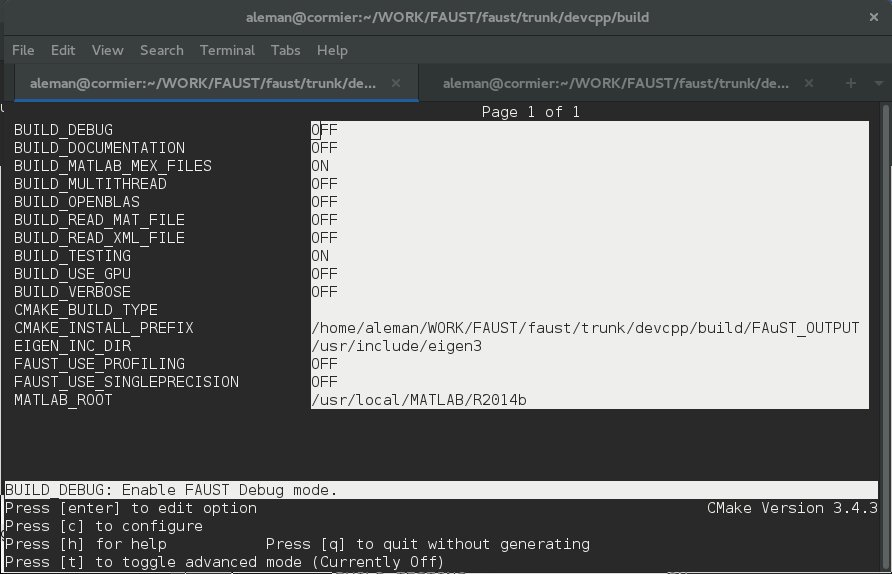
\includegraphics[scale=0.5]{images/ccmake.jpg}
\caption{ccmake GUI}
\label{fig:ccmake}
\end{figure}

\paragraph{}When scrolling on a value and pressing [enter], this value can be edited, the black underlaid row displays some information about the option and required path to create the build system. In the case of an option press [enter] to toggle the ON/OFF values. You can edit option by pressing [enter]. For example, press [enter] to edit option \texttt{CMAKE\_INSTALL\_PREFIX} to modify the install directory. 
\paragraph{}After choosing options for the build and setting the required fields, press [c] to configure. The configuration of the build system is checked again by Cmake, at the end of this check if the build settings are correct, you can press [g] in order to generate the build system.

\paragraph{} Instead the ccmake GUI, an other possibility to configure and generate the project is to use the command line cmake which can take the option input. Here is the list of available options: 
\texttt{cmake\ ..\ -D<BUILD\_NAME>=<value>}

\begin{itemize}
\item CMAKE\_INSTALL\_PREFIX : Install directory
\item BUILD\_TESTING : Enable the ctest option (default value is ON)
\item BUILD\_DOCUMENTATION : Generating the doxygen documentation (default value is OFF)  
\item BUILD\_MULTITHREAD : Enable multithread with OpenMP Multithreading (default value is OFF)
\item BUILD\_VERBOSE : Enable verbose option when compile (-v) (default value is OFF)
\item BUILD\_DEBUG : Enable FA$\mu$ST Debug mode (default value is OFF )
\item BUILD\_USE\_GPU : Using both CPU and GPU process ( default value is OFF)
\item BUILD\_MATLAB\_MEX\_FILES : Enable building Matlab MEX files (default value is ON)
\item BUILD\_OPENBLAS : Using openBLAS for matrix and vector computations (default value is OFF )
\item BUILD\_READ\_XML\_FILE : Using xml2 library to read xml files (default value is OFF)
\item BUILD\_READ\_MAT\_FILE : Using matio library to read mat files (default value is OFF)
\end{itemize}

\paragraph{}Following the selected option, the cmake installer automatically checks the dependent component (library OpenBlas, eigen, matio, libxml2).  

%\section{Optional dependent tools}\label{sec:OptionalRequiredTools}

%\paragraph{Optional Install of GPU process}
%\begin{itemize}
%\item \textbf{Install} CUDA and the drivers for NVIDIA.
%\item \textbf{Verify install} of GPU tools by typing in a terminal : 
%\begin{lstlisting}
%> which nvcc
%\end{lstlisting}
%You must obtain the path of your \texttt{nvcc} compiler like 
%\begin{lstlisting}[backgroundcolor=\color{white}]
%/usr/local/cuda-7.5/bin/nvcc
%\end{lstlisting}
%If not, add \texttt{nvcc} directory in your environment path (in your ~/.bashrc file). 
%\end{itemize}


